\Chapter{Koncepció}

\Section{A fejezet célja}

A szimulációs környezet inspirációt vesz már elkészített játékokból, mint például a Pixel Dungeon és Darkest Dungeon
nevű játékokból ismerhető szoba és folyosó kapcsolat. Ahol minden szobát egy folyosó köt össze egy másik tetszőleges szobával.
A Darkest Dungeon-hoz képest a játékmenet rugalmasabb, mivel a szobák bármikor elhagyhatóak és megközelíthetőek, ha engedi azt a pálya jelenlegi belső felépítése.
Azaz, ha nincs útban valami, ami megakadályozza.

Illetve inspirációt vesz még továbbá a For The King nevezetű játékból, ahol a fegyverek adott karakter statiszkákból "scalelődnek", azaz a birtokolt statiszkák függvényében
számolódnak ki az adott értékek figyelembe véve a célpont általt birtokolt statisztikákat is.

A fent említett három játék mind körökre osztott, ahogyan a szimulációs környezetünk is az lesz.

A szimulációs környezetünk viszont egyedi lesz abból a szempontból, hogy az ágensek csoportokra vannak osztva és közös céllal rendelkezve próbálják legyőzni egymást és a játékost.
Illetve hogy nem csak a játékosnak létezik 'win condition'-je, hanem az ágenseknek is, mindkét frakciónak különböző.

\iffalse
A hivatkozások jelentős része ehhez a fejezethez szokott kötődni.
(Egy hivatkozás például így néz ki \cite{coombs1987markup}.)
Itt lehet bemutatni a hasonló alkalmazásokat.
\fi

\Section{Tartalom és felépítés}

\iffalse
A fejezet tartalma témától függően változhat. Az alábbiakat attól függően különböző arányban tartalmazhatják.
\begin{itemize}
\item Irodalomkutatás. Amennyiben a dolgozat egy módszer kidolgozására, kifejlesztésére irányul, akkor itt lehet részletesen végignézni (módszertani vagy időrendi bontásban), hogy az eddigiekben milyen eredmények születtek a témakörben.
\item Technológia. Mivel jellemzően kutatásról vagy szoftverfejlesztésről van szó, ezért annak a jellemző elemeit, technikai részleteit itt kell bemutatni.
Ez tehát egy módszeres bevezetés ahhoz, hogy ha valaki nem jártas a témakörben, akkor tudja, hogy a dolgozat milyen aktuálisan elérhető eredményeket, eszközöket használt fel.
\item Piackutatás. Bizonyos témáknál új termék vagy szolgáltatás kifejlesztése a cél.
Ekkor érdemes annak alaposan utánanézni, hogy aktuálisan milyen eszközök érhetők el a piacon.
Ez szoftverek esetében a hasonló alkalmazások bemutatását, táblázatos formában történő összehasonlítását jelentheti.
Szerepelhetnek képek és észrevételek a viszonyításként bemutatott alkalmazásokhoz.
\item Követelmény specifikáció. Külön szakaszban érdemes részletesen kitérni az elkészítendő alkalmazással kapcsolatos követelményekre.
Ehhez tartozhatnak forgatókönyvek (\textit{scenario}-k).
A szemléletesség kedvéért lehet hozzájuk képernyőkép vázlatokat is készíteni, vagy a használati eseteket más módon szemléltetni.
\end{itemize}
\fi

\Section{Menü}

A szimuláció indításakor vagy megállításakor felugró ablak.

\begin{itemize}
    \item Start/Continue:
    A szimuláció indításakor a menüben a start-ot látjuk, ha a szimulációt állítjuk meg, akkor a menüben a continue-t látjuk.
    Ezen menüpont kiválasztásával kezdhetjük a szimulációt vagy folytathatjuk azt.
    \item Save:
    Ez a menüpont nem jelenik meg a szimuláció indításakor csak akkor, hogyha szimulációt állítunk meg.
    Ezen menüpont kiválasztásával menthetjük a jelenlegi szimulációnkat.
    \item Load:
    Ezen menüpont mindig jelen van a menüben, elérhető a szimuláció indításakor és megállításakor is.
    Ezen menüpont kiválasztásával tölthetjük be az általunk lementett mentéseket.
    \item Options:
    Ezen menüpont mindig jelen van a menüben, elérhető a szimuláció indításakor és megállításakor is.
    Ezen menüpont kiválasztásával egy új ablakra irányít át minket.
    Itt lehetőségünk van hangbeállítások személyre szabására, mint például a zene és a szimulációbeli hangok. (Több csúszka segítségével)
    Lehetőségünk van fényerő beállításokra is, mint például a Gamma állítására. (Egy csúszka segítségével)
    Nyelvi beállítások a menüre vonatkozóan. (Legördülő fülből kiválasztva)
    Végezetül egy visszagomb ami visszairányít minket a menübe.
    \item Log out:
    Kiléptet minket a jelenlegi fiókunkból, visszairányítva a bejelentkezési ablakhoz.
    A log-out a menüben mindig szerepel.
    \item Main menu:
    Ez a gomb akkor szerepel a menüben hogyha egy szimuláció megállításával kerülünk a menübe.
    Ez befejezi a jelenlegi szimulációnkat és visszaírányít minket a főmenübe.
\end{itemize}

\Section{Szimulációs környezet specifikálása}

\subsection{Szobák és folyosók}

A szobákat több szomszédos cellák alkotják, ezeket a szobákat folyosók kötik össze, amelyeket pontosan kettő cellával szomszédos cellák alkotnak.
Minden szomszédos szobát és folyósót egy ajtó választ el egymástól.
Celláin korlátozottan helyezkedhetnek el térbeli objektumok(Lásd: oszlop), amely a cellát nem bejárható cellává alakít és korlátozza a látást.

\subsection{Map}

A map szobák és folyosók összesége, ahol a szobák alakjánál törekszünk a négyzet alakú szobák elkerülésére. A folyosók általában rövidek és egy szóbából akár több is nyílik egy adott szobára.
A szobákban és a folyosókban bejárható terület egy mátrixhoz hasonló, ahol a celláit blokkoknak nevezzük.
Minden blokkhoz tartoznak adatok.

\noindent Ezek az adatok:

\begin{itemize}
    \item X koordináta (egészérték),
    \item Y koordináta (egészérték),
    \item Entity (intiger típusú érték,  az adott blokkon lévő entity ID-ját tartalmazza),
    \item Tárgy (integer típusú tömb, az adott blokkon lévő tárgyak ID-ját tartalmazza),
    \item Effect (többértékű összetett tulajdonság, tartalmazza az EffectIDt és EffectTimeot),
    \item EffectID (integer típusú tömb, az adott blokkon lévő effektek ID-ját tartalmazza),
    \item EffectTime (integer típusú tömb, az adott blokkon lévő effektek lejárási idejét tartalmazza).
\end{itemize}

\noindent Fontosabb kizáró feltételek:

\begin{itemize}
    \item Ajtó csak szoba és a folyosó, vagy szoba és a szoba között létezzen.
    \item Folyosóból ne nyíljon ajtó folyosóra.
    \item Két különböző folyósó ne érjen össze.
    \item Minden szobából nyíljon ajtó, úgy hogy lehetséges legyen elhagyni.
    \item A map bármelyik részéből elérhető legyen a map bármelyik tetszőleges helye.
    \item Folyosó ne legyen eltorlaszolva nem bejárható térbeli objektummal, mint például: Oszlop.
\end{itemize}

\Section{Karakterünk}

\subsection{Szint}

Karakterünk rendelkezik egy szinttel, ami a legelején az 1es szintről indul.
Entity legyőzése ad karakterünknek tapasztalatpontot, amelyből ha megszerzünk egy adott mennyiséget, a karaktünk szintet lép.
Minden következő szinthez 10\%-kal több tapasztalatpont szükséges, mint az előző szinthez.
Szintlépéskor lehetőségünk van a Karakter oldalon a szintlépéskor kapott 3 pontunkat elosztani a fő 4 statisztikára.(Lásd: Statisztika)

\subsection{Statisztika}

Entityk és karakterünk 4 alap statisztikával rendelkezik.
Ez a 4 statisztika a következők: Erő, Kitérés, Kitartás, Pontosság.

\noindent Kezdő statisztika:
\begin{itemize}
    \item Erő: 10
    \item Kitérés: 10
    \item Kitartás: 10
    \item Pontosság: 10
\end{itemize}

\Section{Ágensek}

\subsection{Tolvaj}

\noindent Kezdő statisztika:
\begin{itemize}
    \item Erő: 8
    \item Kitérés: 12
    \item Kitartás: 8
    \item Pontosság: 12
\end{itemize}

\subsection{Harcos}

\noindent Kezdő statisztika:
\begin{itemize}
    \item Erő: 12
    \item Kitérés: 8
    \item Kitartás: 12
    \item Pontosság: 8
\end{itemize}

\subsection{Sebzés számlálás}

...

\subsection{Kommunikáció közöttük}

Az Entityk, ahogyan mi is, maguk elé 3 szélességben és 4 hosszúságnyi téglalapot látnak, illetve a karakter állásától 90fokra mindkét oldalra homályosan látnak 2 cellányit előre.
Megfigyelik, hogy:
\begin{itemize}
    \item Eldöntik, hogy elégségesen ismerik-e környezetüket
    \item Nyitva vannak-e az ajtók
    \item Merre mennek az Entityk és a játékos
    \item Vannak-e hátrahagyott elpusztult Entityk
    \item Nyitva vannak-e a ládák
    \item Megszerezték-e a győzelemhez szükséges Tárgyat
    \item Látják-e őt az ellenséges Entityk vagy a játékos
\end{itemize}

\subsection{Megfigyelési akcióik}

Hogyan reagálnak az általuk nyert információkra?
\begin{itemize}
    \item Ha úgy itéli meg, hogy környezetét nem ismeri eléggé, Körbetekintés segítségével felfedezi környezetét.
    \item Ha nyitva vannak-e az ajtók és nem tudják mely Entity által, akkor körbenézhetnek, hogy megtalálják a tettest.
    \item Ha tudják merre mennek az Entityk és a játékos, aszerint tervezik útvonalokat, vagy támadnak
    \item Ha vannak hátrahagyott elpusztult Entityk, amelyek nem rég nem voltak ott, akkor körbenézhetnek, hogy megtalálják a tettest.
    \item Ha nyitva vannak a ládák, amelyek nem rég nem voltak nyitva, akkor körbenézhetnek, hogy megtalálják a tettest.
    \item Ha Megszerezték a győzelemhez szükséges Tárgyat, akkor támogatják csapattársaikat, ha más szerezte meg, megpróbálják megakadályozni.
    \item Ha nem látják ellenséges Entityk vagy játékos, de ők látják, megpróbálnak mögé ossoni és hátból támadni váratlanul.
\end{itemize}

\subsection{Elérendő céljaik}

...

\Section{Effektek}

Effektek típusai:
\begin{itemize}
    \item Pozitív,
    \item Negatív.
\end{itemize}
Effektek cellákon vagy karaktereken elhasználva 3 körig léteznek.

\subsection{Pozitív Effektek}

\begin{itemize}
    \item Vigor: maximum HP 5\% visszatöltés.
    \item Steel: Sebzés számoláskor 30\%-kal kevesebb sebzés elszenvedés.
\end{itemize}

\subsection{Negatív Effektek}

\begin{itemize}
    \item Poison: maximum HP 5\% elvesztése.
    \item Weakness: Sebzés számoláskor a Kitérés statisztika 30\%-kájának ignorlása.
\end{itemize}

\Section{Combat}

A szimulációban Entity és Entity vagy Entity és karakter közötti HP elvétel lehetséges,
\begin{itemize}
    \item szomszédos cellából támadás által(Lásd: támadás),
    \item azonos X vagy Y koordinátájú cellából statisztikák által meghatározott távolságnyira dobás által(Lásd: dobás),
    \item cellák effekt tulajdonságának manipulálciója(Lásd:Effektet változtató tárgyak eldobása), effektek által,
    \item csapdák által, amelyek a játék kezdetekor generálódtak.
\end{itemize}


\Section{Tárgyak}

A tárgyakhoz a következő adatok tartoznak:
\begin{itemize}
    \item ItemID
    \item ItemName
    \item ItemType
    \item Quantity
    \item MaxQuantity
\end{itemize}

\subsection{ItemID}

A tárgyak generálásakor minden tárgy kap egy egyedi ID-t, ez az ID határozza meg, hogy statisztikái milyennek lettek legenerálva az adott nyílt intervallumon belül.
A karakterre felszerelhető tárgyak értékei randomizáltak, a map generálaskor döntődnek el egy adott nyílt intervallumon belül.

\subsection{ItemName}

A tárgyak tartalmaznak tárgynevet, azonos nevű tárgyak tulajdonságainak értékei azonos nyílt intervallumon belül generáltak.

\subsection{ItemType}

A tárgyak típusai a szimulátorban a következők lehetnek:
\begin{itemize}
    \item Inventoryból használható tárgyak(körért),
    \item Karakterre felszerelhető tárgyak(körért),
    \item Adott célra használható tárgyak(Lásd: Kulcs, CélTárgy).
\end{itemize}

\subsection{Quantity}

A tárgyak Quantity adatja azt az integer számot tartalmazza, amennyi létezik az inventoryban.

\subsection{MaxQuantity}

A tárgyak MaxQuantity értéke azt határozza meg, mennyire stackelhet fel egy adott Item az inventoryban, ha túllépi a MaxQuantity számát, akkor új stack-et kezd.

\Section{Tárgy nevek}

\subsection{Vigor Flask}

Entity elpusztulásakor az adott cellán hagyja hátra 5\%-os eséllyel, de egyszerre csak háromnál kevesebbet hagyhat hátra.

\noindent Elérhető interakciók:
\begin{itemize}
    \item Használat: Adott karakteren 3 körig érvényesül a Vigor effekt.(Lásd Effektek)
    \item Eldobás: Adott cellán 3 körig érvényesül a Vigor effekt.(Lásd Effektek)
\end{itemize}

\subsection{Steel Flask}

Entity elpusztulásakor az adott cellán hagyja hátra 5\%-os eséllyel, de egyszerre csak háromnál kevesebbet hagyhat hátra.

\noindent Elérhető interakciók:
\begin{itemize}
    \item Használat: Adott karakteren 3 körig érvényesül a Steel effekt.(Lásd Effektek)
    \item Eldobás: Adott cellán 3 körig érvényesül a Steel effekt.(Lásd Effektek)
\end{itemize}

\subsection{Poison Flask}

Entity elpusztulásakor az adott cellán hagyja hátra 5\%-os eséllyel, de egyszerre csak háromnál kevesebbet hagyhat hátra.

\noindent Elérhető interakciók:
\begin{itemize}
    \item Használat: Adott karakteren 3 körig érvényesül a Poison effekt.(Lásd Effektek)
    \item Eldobás: Adott cellán 3 körig érvényesül a Poison effekt.(Lásd Effektek)
\end{itemize}

\subsection{Weakness Flask}

Entity elpusztulásakor az adott cellán hagyja hátra 5\%-os eséllyel, de egyszerre csak háromnál kevesebbet hagyhat hátra.

\noindent Elérhető interakciók:
\begin{itemize}
    \item Használat: Adott karakteren 3 körig érvényesül a Weakness effekt.(Lásd Effektek)
    \item Eldobás: Adott cellán 3 körig érvényesül a Weakness effekt.(Lásd Effektek)
\end{itemize}

\subsection{Entity Helm no.1}

Entity elpusztulásakor az adott cellán hagyja hátra 10\%-os eséllyel, de egyszerre csak egy tárgyat hagyhat hátra.
Játékos által használható felszerelési tárgy, amely pozitív és negatív statisztikát ad, amelyek hozzáadódnak, illetve kivonódnak a játékos jelenlegi statisztikáiból.

\begin{itemize}
    \item Erő: ]2,4[
    \item Kitérés: ]-2,-4[
    \item Kitartás: ]2,4[
    \item Pontosság: ]-2,-4[
\end{itemize}

\subsection{Entity Helm no.2}

Entity elpusztulásakor az adott cellán hagyja hátra 10\%-os eséllyel, de egyszerre csak egy tárgyat hagyhat hátra.
Játékos által használható felszerelési tárgy, amely pozitív és negatív statisztikát ad, amelyek hozzáadódnak, illetve kivonódnak a játékos jelenlegi statisztikáiból.

\begin{itemize}
    \item Erő: ]-2,-4[
    \item Kitérés: ]2,4[
    \item Kitartás: ]-2,-4[
    \item Pontosság: ]2,4[
\end{itemize}

\subsection{Entity Armor no.1}

Entity elpusztulásakor az adott cellán hagyja hátra 10\%-os eséllyel, de egyszerre csak egy tárgyat hagyhat hátra.
Játékos által használható felszerelési tárgy, amely pozitív és negatív statisztikát ad, amelyek hozzáadódnak, illetve kivonódnak a játékos jelenlegi statisztikáiból.

\begin{itemize}
    \item Erő: ]2,4[
    \item Kitérés: ]-2,-4[
    \item Kitartás: ]2,4[
    \item Pontosság: ]-2,-4[
\end{itemize}

\subsection{Entity Armor no.2}

Entity elpusztulásakor az adott cellán hagyja hátra 10\%-os eséllyel, de egyszerre csak egy tárgyat hagyhat hátra.
Játékos által használható felszerelési tárgy, amely pozitív és negatív statisztikát ad, amelyek hozzáadódnak, illetve kivonódnak a játékos jelenlegi statisztikáiból.

\begin{itemize}
    \item Erő: ]-2,-4[
    \item Kitérés: ]2,4[
    \item Kitartás: ]-2,-4[
    \item Pontosság: ]2,4[
\end{itemize}

\subsection{Entity Weapon no.1}

Entity elpusztulásakor az adott cellán hagyja hátra 10\%-os eséllyel, de egyszerre csak egy tárgyat hagyhat hátra.
Játékos által használható felszerelési tárgy, amely pozitív és negatív statisztikát ad, amelyek hozzáadódnak, illetve kivonódnak a játékos jelenlegi statisztikáiból.

\begin{itemize}
    \item Erő: ]1,5[
    \item Kitérés: ]-1,-3[
    \item Kitartás: ]0,-1[
    \item Pontosság: ]-1,2[
\end{itemize}

\subsection{Entity Weapon no.2}

Entity elpusztulásakor az adott cellán hagyja hátra 10\%-os eséllyel, de egyszerre csak egy tárgyat hagyhat hátra.
Játékos által használható felszerelési tárgy, amely pozitív és negatív statisztikát ad, amelyek hozzáadódnak, illetve kivonódnak a játékos jelenlegi statisztikáiból.

\begin{itemize}
    \item Erő: ]-1,2[
    \item Kitérés: ]1,3[
    \item Kitartás: 0
    \item Pontosság: ]1,5[
\end{itemize}

\subsection{Kulcs}

Vagy Entityktől, vagy celláról szerezhetőek meg.
Szerepük a ládák kinyitása a játékos által.

\subsection{Cél Tárgy}

Map teljesítéséhez szükséges tárgy.

\Section{Interface felület}

\subsection{Menü}

\begin{itemize}
    \item prekondíció: A szimulációs ablakban vagyunk.
    \item általános működés: Rávisszük az egeret, majd bal kattintással megnyitjuk.
    \item alternatív esetek: Rossz menü ablak nyílik meg.
    \item Postkondíció: Megnyílt a menü ablak.
    \item kivételes esetek: Nem nyílt meg az ablak.
\end{itemize}

\subsection{Inventory}

\begin{itemize}
    \item prekondíció: A szimulációs ablakban vagyunk.
    \item általános működés: Rávisszük az egeret, majd bal kattintással megnyitjuk.
    \item alternatív esetek: Rossz ablak nyílik meg.
    \item Postkondíció: Megnyílt az inventory ablak.
    \item kivételes esetek: Nem nyílt meg az ablak.
\end{itemize}

\subsection{Map}

\begin{itemize}
    \item prekondíció: A szimulációs ablakban vagyunk.
    \item általános működés: Rávisszük az egeret, majd bal kattintással megnyitjuk.
    \item alternatív esetek: Rossz ablak nyílik meg.
    \item Postkondíció: Megnyílt a Map ablak.
    \item kivételes esetek: Nem nyílt meg az ablak.
\end{itemize}

\subsection{Karakter}

\begin{itemize}
    \item prekondíció: A szimulációs ablakban vagyunk.
    \item általános működés: Rávisszük az egeret, majd bal kattintással megnyitjuk.
    \item alternatív esetek: Rossz ablak nyílik meg.
    \item Postkondíció: Megnyílt a Karakter ablak.
    \item kivételes esetek: Nem nyílt meg az ablak.
\end{itemize}

\subsection{Dobás}

\begin{itemize}
    \item prekondíció: A szimulációs ablakban vagyunk.
    \item általános működés: Rávisszük az egeret, majd bal kattintás után kiválasztjuk a dobandó Tárgyat, és a cél cellát(maximum választható hosszúság a statisztikák alapján számolódik ki).
    \item alternatív esetek: Rossz tárgyat dob el.
    \item Postkondíció: Eldobtuk az adott tárgyat a célbavett cellára, ha a cella tartalmaz Entity, akkor kiszámolódik az új HP mennyiség, az Inventoryban ha dobás előtti Quantity 1-nél több, akkor 1 levonódik belőle. Végül átadtuk a kört.
    \item kivételes esetek: Nem dobta el a Tárgyat.
\end{itemize}

\subsection{Felvétel}

\begin{itemize}
    \item prekondíció: A szimulációs ablakban vagyunk és a karakterünk celláján létezik valamilyen tárgy.
    \item általános működés: Rávisszük az egeret, majd bal kattintással felvesszük a Tárgyat, ha kiválaszottuk melyik Tárgyat vesszük fel a bal és jobbra mutató nyilak segítségével.
    \item alternatív esetek: Rossz Tárgyat vesz fel.
    \item Postkondíció: Felvettük a kiválasztott Tárgyat. Ha már szerepelt azonos nevű Tárgy az Inventoryban és a maxQuantity nem érte el a maximumát, akkor Quantity-hez hozzáadódik 1, máskülönben új stacket kezd az inventoryban.
    \item kivételes esetek: Nem vette fel a Tárgyat.
\end{itemize}

\subsection{Körbetekintés}

\begin{itemize}
    \item prekondíció: A szimulációs ablakban vagyunk.
    \item általános működés: Rávisszük az egeret, majd bal kattintással elindítjuk a folyamatot.
    \item alternatív esetek: Nem kapunk rálátást a körbeforgott területre.
    \item Postkondíció: Rálátást nyertünk a környezetünkre, mintha minden irányban látnánk és elhasználtuk a körünket.
    \item kivételes esetek: Nem fordult körbe a karakter.
\end{itemize}

\subsection{Láda nyitás}

\begin{itemize}
    \item prekondíció: Ládát tartalmazó cellához vízszintesen vagy függőlegesen közvetlen szomszédos cellán tartózkodunk.
    \item általános működés: Rávisszük az egeret a felbukkanó ikonra, majd bal kattintással elindítjuk a folyamatot.
    \item alternatív esetek: Nem tartalmaz semmit a láda.
    \item Postkondíció: Kinyílt a láda, az adott tárgyat megkaptuk.
    \item kivételes esetek: Nem nyílt ki a láda.
\end{itemize}

\subsection{Támadás}

\begin{itemize}
    \item prekondíció: A szimulációban a karakterünk cellájához szomszédos cella tartalmaz Entity.
    \item általános működés: Rávisszük az egeret a felbukkanó ikonra, majd bal kattintással elindítjuk a folyamatot.
    \item alternatív esetek: Nem támad a karakterünk.
    \item Postkondíció: A támadás végbe ment, és kiszámításra került a célpont új HP mennyisége.
    \item kivételes esetek: Nem számolodott ki az új HP mennyiség.
\end{itemize}

\Section{Mapon található mozgást kizáró objektumok}

\subsection{Láda}

A ládák map generáláskor kerülnek bizonyos cellákra.
Entityk dobják a kulcsukat, vagy a mapra generálódik le valamelyik cellára.
Ládát tartalmazó cellára nem lehetséges a mozgás.
Interakcióval kinyitható, ha az Inventory tartalmazza a kulcsát. (Lásd: Interface)

\subsection{Oszlop}

Az oszlopok map generáláskor kerülnek bizonyos cellákra.
Oszlopoknak semmilyen különleges funkciója nincs azonkívül, hogy map komplexitását kívánja növelni azzal,
hogy mozgást és látást korlátozó szerepet lát el.

\subsection{Zárt ajtó}

Az ajtók map generáláskor kerülnek csak olyan cellákra, ahol egy szobából egy folyosón lehetséges elhagyni a szobát.
Mindig zárt alakban kerül az adott cellákra, kinyitásához nem szükséges semmilyen különleges tárgy. Ha bármely karakter egy ajtót tartalmazó cellára lép, az ajtó kinyílik amíg Entityt tartalmaz az adott cella.
Ahogyan az Oszlopok, a zárt ajtók is map komplexitását kívánja növelni azzal,hogy látást korlátozó szerepet lát el.

\Section{Idő}

Az idő a szimuláción belül minden általunk végrehajtott akció által telik.
Ha elvégzünk egy akciót, akkor az irányítás átkerül egy másik Entityre,
ami végig megy minden Entity, és ha végig ment a sor, akkor újra mi következünk.

\Section{Kamera}

A kamera normál esetben a karakterünk felett helyezkedik el, és ezáltal tekinthetünk le a map.
A kamera használható korlátozottan szabad módban is, ahol a kamera elrugaszkodik a karakterünktől, és körbe nézhetünk.

\Section{Láthatóság}

Az általunk nem felfedezett map részek, semmilyen módon nem láthatóak általunk, ha már egyszer bejártuk az adott területet, 
de nem látja a karakterünk, akkor csak a terület alakját láthatjuk, az adott cellák frissülését(Lásd: Új Entity megjelenése) már nem fogjuk látni.

\Section{Irányítás}

\begin{itemize}
    \item Kamera szabad mód be- és kikapcsolása: SPACE
    \item Kamera szabadmódbna mozgatása: WASD
    \item A szimulációs térben karakterünk mozgásra utasítása: LEFT CLICK (általunk már felfedezett cellára)
    \item A Menü megnyitása: ESCAPE
    \item Az Inventory megnyitása: I
    \item Map megnyitása: M
    \item Karakter oldal megnyitása: K
\end{itemize}

\begin{figure}[!ht]
	\centering
	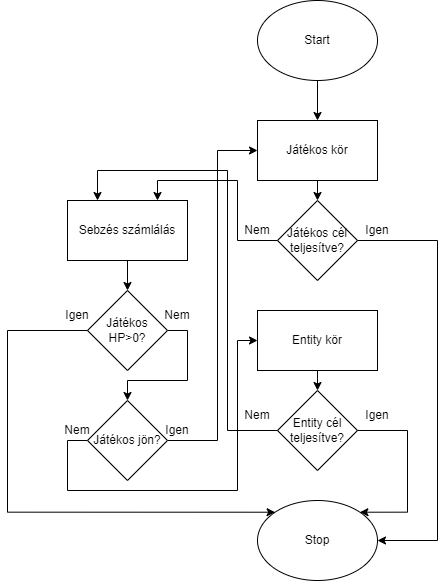
\includegraphics[scale=0.8]{images/gameUML.png}
	\caption{Base Simulation}
	\label{fig:basegame}
\end{figure}

\begin{figure}[!ht]
	\centering
	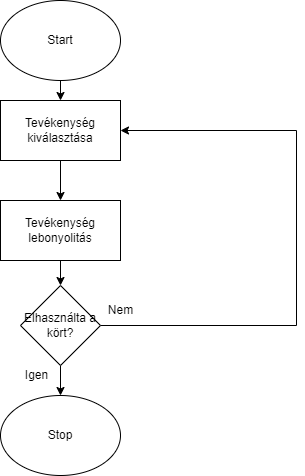
\includegraphics[scale=1]{images/playerturnUML.png}
	\caption{Player Turn}
	\label{fig:playerturn}
\end{figure}

\begin{figure}[!ht]
	\centering
	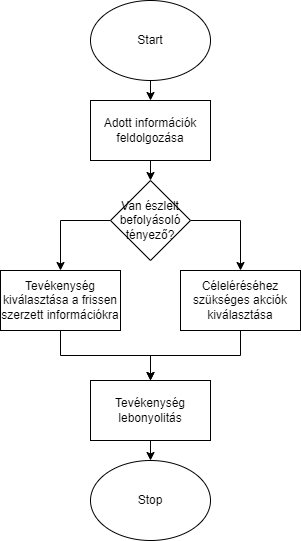
\includegraphics[scale=1]{images/entityturnUML.png}
	\caption{Entity Turn}
	\label{fig:entityturn}
\end{figure}

\begin{figure}[!ht]
	\centering
	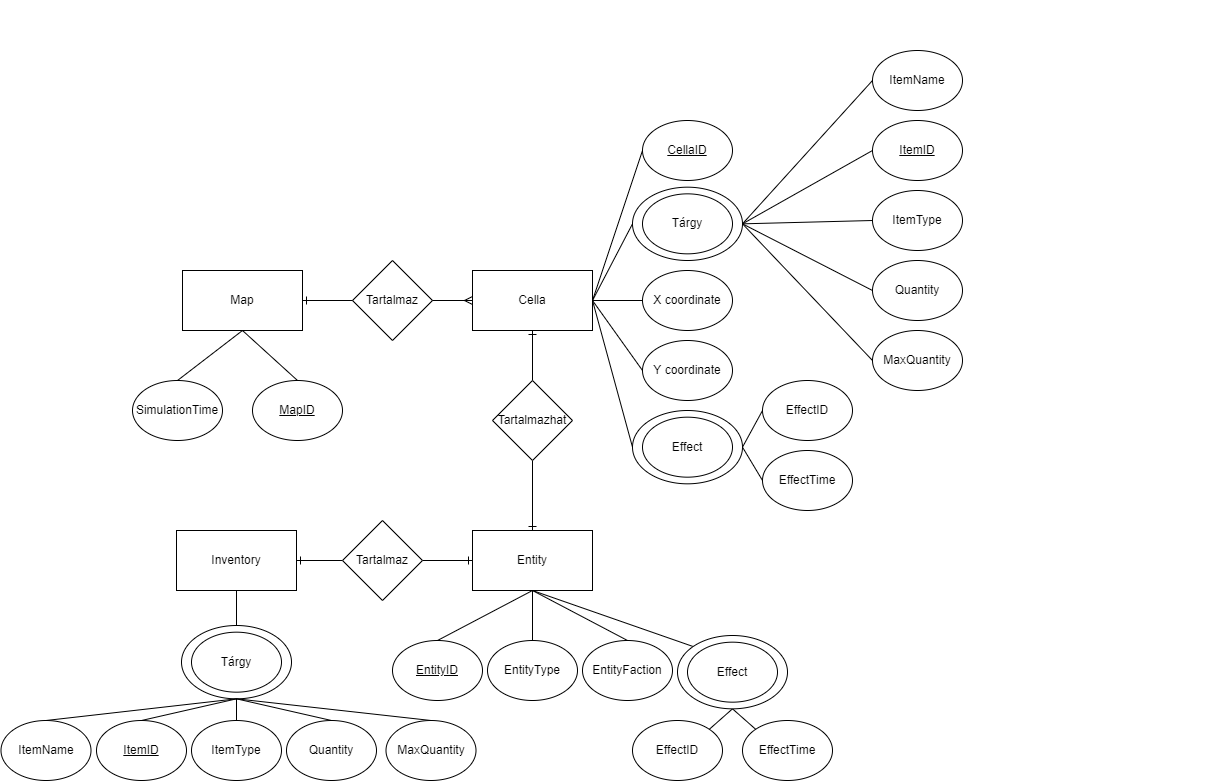
\includegraphics[scale=0.4]{images/simulationER.png}
	\caption{Simulation}
	\label{fig:simulation}
\end{figure}

